% Chapter 8

\chapter{Graphical User Interface - GUI} % Main chapter title

\label{Chapter7} % For referencing the chapter elsewhere, use \ref{Chapter1} 

\lhead{Chapter 7. \emph{GUI}} % This is for the header on each page - perhaps a shortened title

%----------------------------------------------------------------------------------------
\section{C++}
\subsection{Framework choice}

For UI in this project we have chosen to use Qt Widgets Module. Qt features two technologies for creating desktop user interfaces. The first choice for this project was Qt Quick, since it provides the most appropriate functionality to mimic Google Earth web-application look and feel with fluid and dynamic user interface. However, the development process was very slow and difficult due to the fact that Qt Quick is rather new technology and not well-documented. It turned out to be more feasible to use older and more reliable technology, Qt Widgets. Qt Widgets are mature and feature rich user interface elements suitable for mostly static user interfaces. Besides, since Qt Widget are native C++ elements it is easier to merge UI with the application logic.
The application UI is connected to all other parts of the application through the class Logic.  The Logic handles all the data interchange between the UI, database and algorithms. In this was it is possible to split the application in separate parts. 

\subsection{Basic elements of UI}

The UI is straightforward and easy to use. There are two main parts - control panel and map. It is possible to extract three multiple cases of the application usage from the task: the search of Point-to-Point shortest path; the search of the destination in the given radius; the itinerary search with the middle point given as any from the category. Thus, the control contains three tabs corresponding to the three different functions. In each of them there are three options to enter the start and end point; you can either directly use geographical coordinates, choose from the category and POI, or by click on the map. Clicking on the map can have two effects: if you clock in the vicinity of the POI it will be chosen as start/end point, otherwise, just coordinates of the point clicked on the map will be set.
After user have chosen all the parameters of the search, the button "Go!" calls path searching algorithms. The important part is to check that inputs are valid and satisfy bounding conditions of the map. Then the result is displayed with graphical functions and text output.
 \begin{figure}[h]
 \centering
 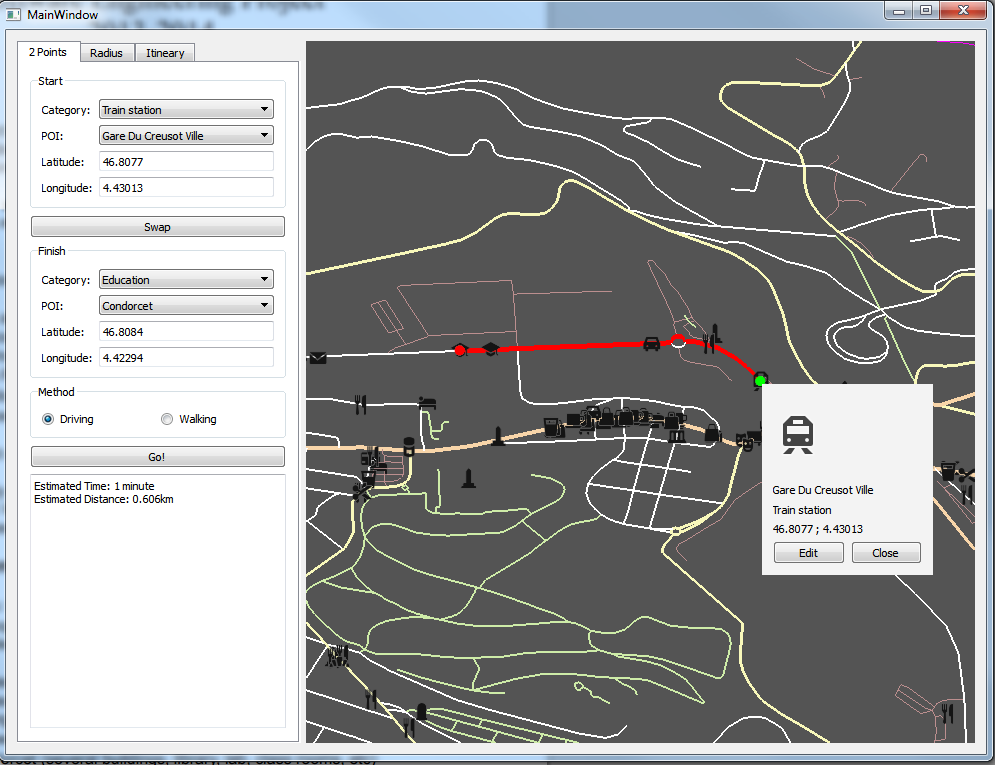
\includegraphics[ width=0.8\textwidth]{../pictures/2point_3.png}
 \caption{How much time does it take to drive from the train station to Condorcet?}
 \end{figure}
  \begin{figure}[h]
  \centering
  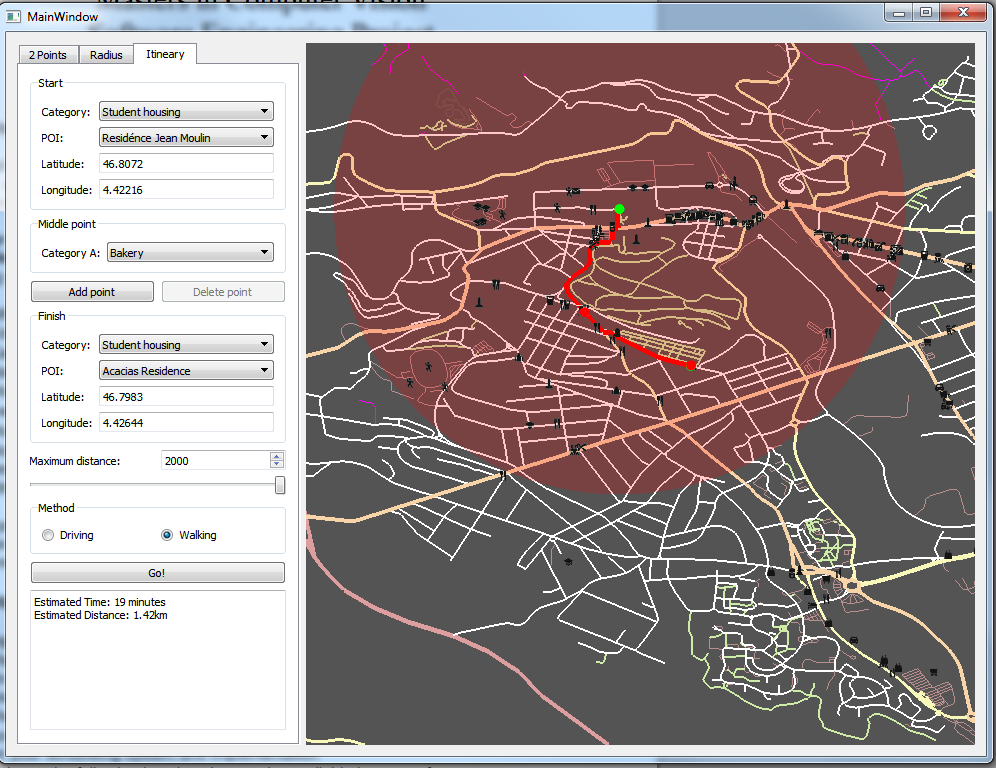
\includegraphics[ width=0.8\textwidth]{../pictures/Radius_0.png}
  \caption{Can you provide an itinerary that is at most 5km long, that passes by a bakery, that 
  starts in Résidence Jean Moulin, and that ends in the Résidence Acacia?}
  \end{figure}


\subsection{Editing the POI database}

The POI can be seen on the map as various descriptive icons according to the category they belong to. Once user clicks on one of the POI small widget appears with the details of the POI. If "Edit" button is pressed, you can edit any data belonging to the chosen POI. Besides user can add POI by choosing one on the options in the context menu, which appears with on-map mouse click. 
 
  \begin{figure}[h]
  \centering
  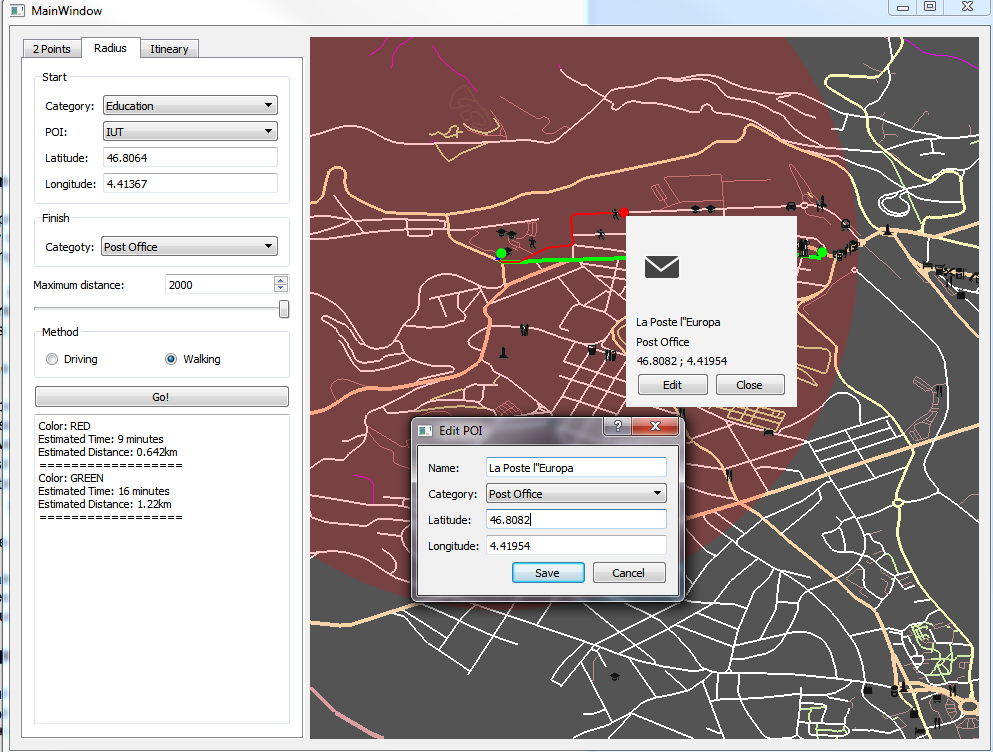
\includegraphics[ width=0.8\textwidth]{../pictures/EditPOI.png}
  \caption{Editing Existing POI}
  \end{figure}
  
    \begin{figure}[h]
    \centering
    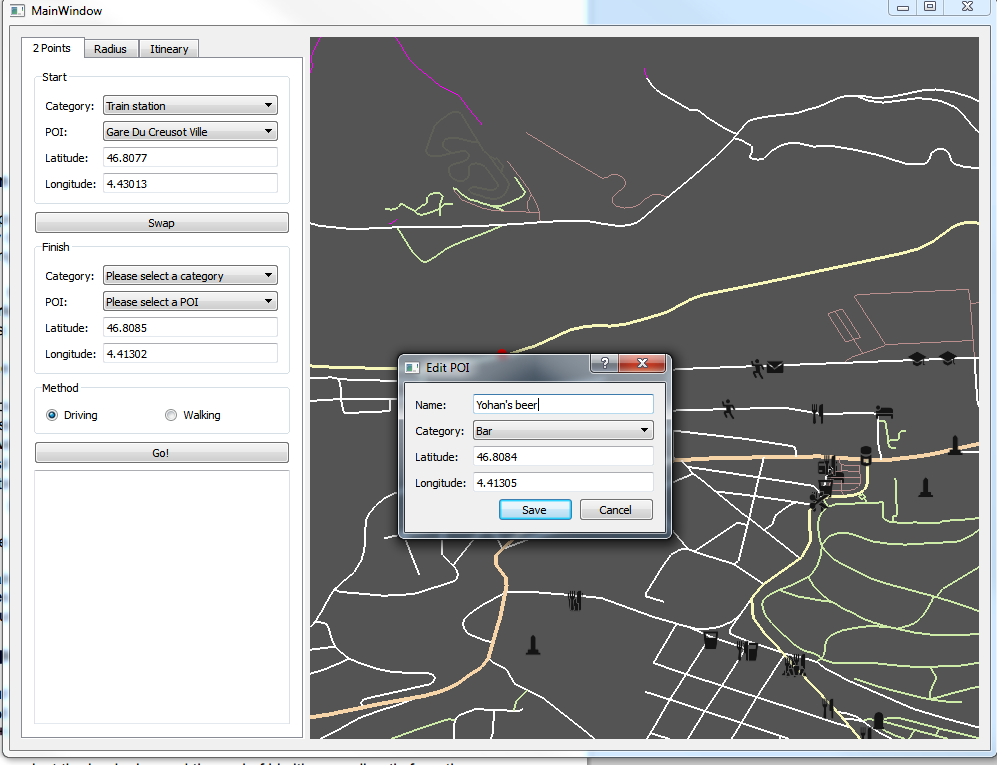
\includegraphics[ width=0.8\textwidth]{../pictures/AddPOI.png}
    \caption{Adding new POI}

    \end{figure}
    
\section{Matlab}
	Graphical user interface is main connection link between user and the program. By the correctly representation of data in GUI user can get all information that he needs. That is why it is so important to implement user interface that from the one hand will be easily understandable by user, and on the another hand can represent all possibilities of the program. In this chapter we will represent GUI for C++ and Matlab part, discuss its main features and difficulties.
	
	\subsection{MATLAB GUI}
	
		\subsubsection{Creating GUI with GUIDE Layout Editor}
			For creation GUI in MATLAB the GUIDE Layout Editor was used. It allows design graphically user interface and then generates code that corresponds to each element of the user interface. GUI can be consists of standard elements like axes, toggle buttons, push buttons, panels and others.\\
			
			Yomap MATLAB GUI is represented on figure \ref{fig:721} and consists from next elements:
			\begin{itemize}
				\item figure
				\item axes
				\item panels
				\item textboxes
				\item checkboxes
				\item toggle buttons
				\item push button
				\item static text
				\item pop-up menus
			\end{itemize}
			
			\begin{figure}[h]
			\centering
			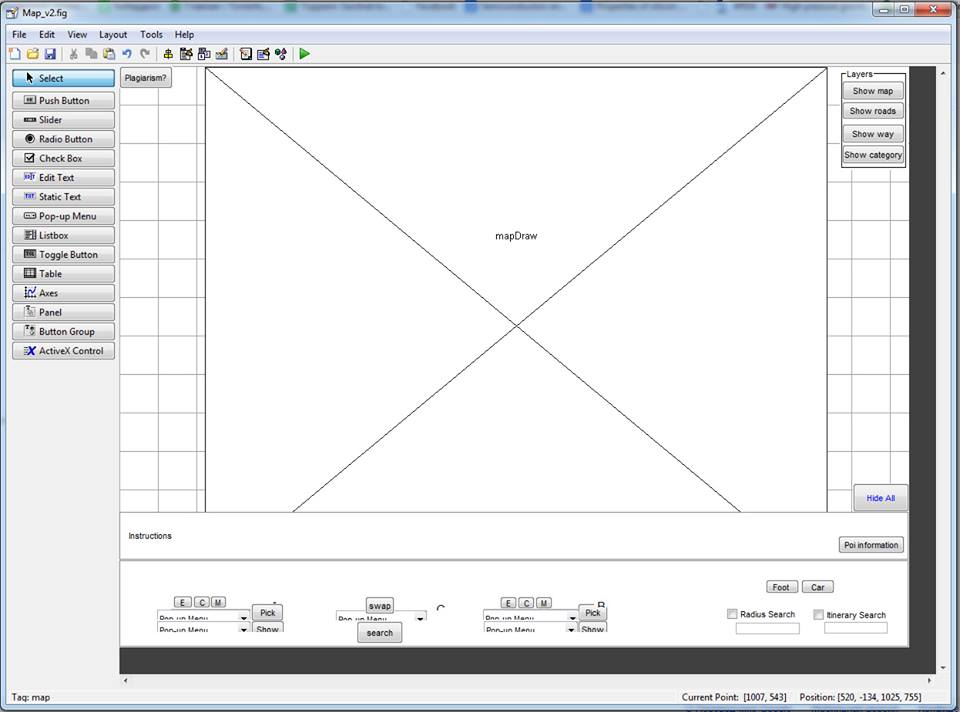
\includegraphics[ width=0.8\textwidth]{../pictures/721.jpg}
			\caption{ Yomap GUI representation in GUIDE Layout Editor}
						\label{fig:721}
			\end{figure}
			The final result of GUI is represented on figure \ref{fig:722} and has such functionality: 
			\begin{itemize}
				\item Zooming map in
				\item Zooming map out
				\item Pan map
				\item Plotting map layers
				\item Picking points on map with mouse click
				\item Choosing categories and points of interest by choosing from pop-up menu
				\item Choosing categories and points of interest with mouse click
				\item Enter name and address of the points of interest
				\item Enter coordinates of the points of interest
				\item Enable/disable middle point
				\item Hide/show search panel
				\item Show point of interest information
				\item Swapping points
				\item Choosing type of transport  
			\end{itemize}
			
			    \begin{figure}[h]
			    \centering
			    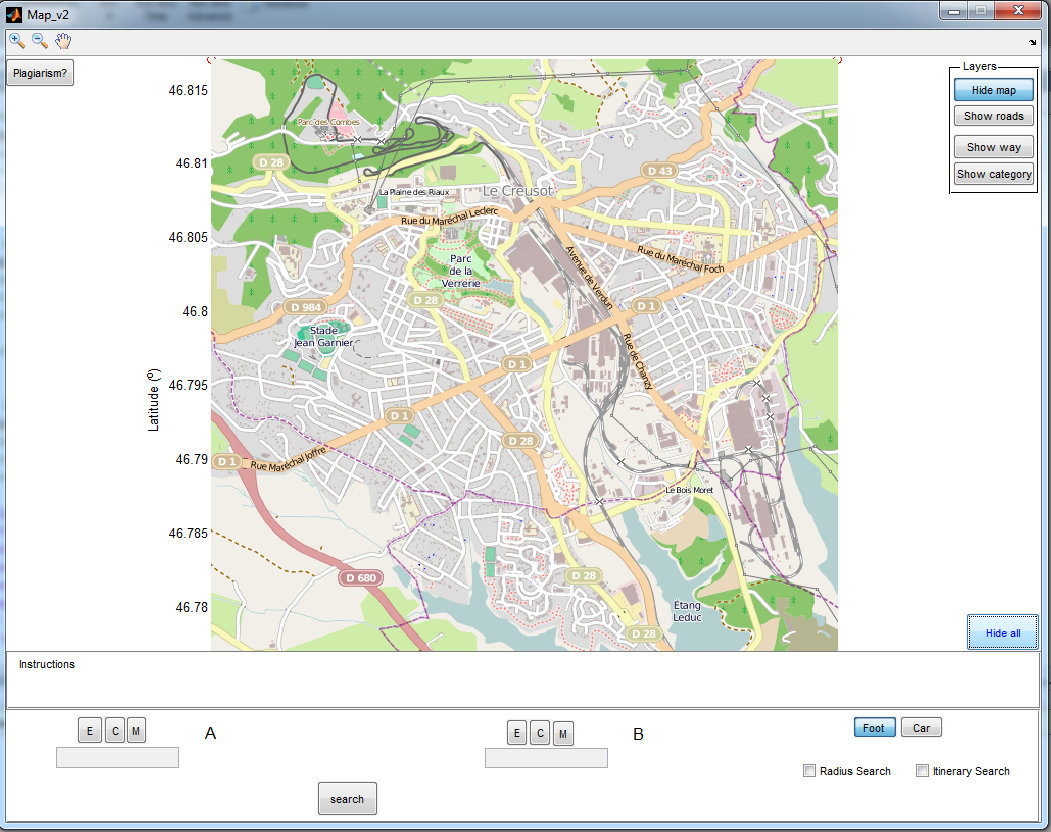
\includegraphics[ width=0.8\textwidth]{../pictures/722.jpg}
			    \caption{Yomap GUI}
				\label{fig:722}
			    \end{figure}
			
			For zooming in, zooming out and pan map standard MATLAB functions were used. For others features callback functions were used. 
			User is allowed to enter name or coordinates of point of interest manually or with mouse click. In case of typing all information into text boxes it is verified and in case of error corresponding message is appear. If user prefers use mouse click coordinates are checking on being in range of the map.
			Another feature of the Yomap GUI is hiding/showing search panel (figure \ref{fig:723}). Because sizes of the map are not allowed to show map and search panel together on the screens with small resolutions we decided to hide a panel for better map representation. In case if button “Hide All” is pressed the search panel became invisible and panel with instructions moves to the bottom of graphic window to show the whole map. After pressing button again all panels appear back on their initial places. 
			
			  \begin{figure}[h]
			  \centering
			  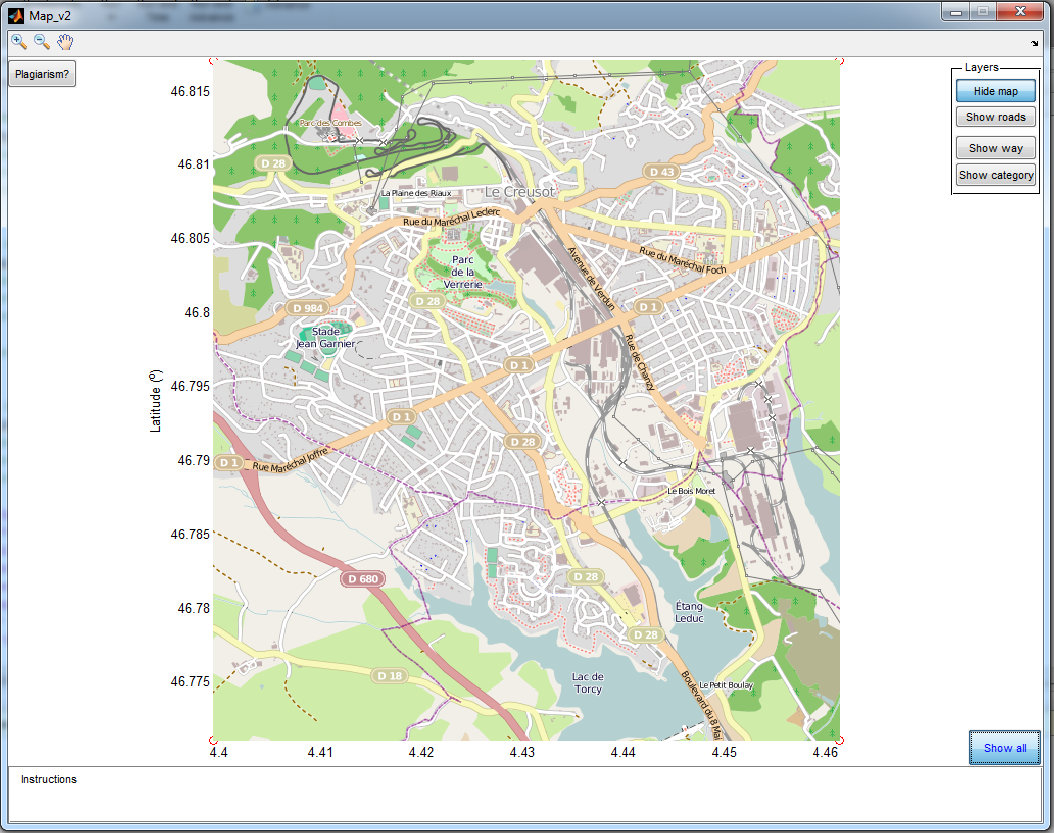
\includegraphics[ width=0.8\textwidth]{../pictures/723.jpg}
			  \caption{Yomap GUI search panel}
			\label{fig:723}
			  \end{figure}
			
			For user convenience button “swap” was implemented (figure \ref{fig:724}). In case of the same type of point of interest representation after pressing button “swap” all information between two points changes.  
			  \begin{figure}[h]
			  \centering
			  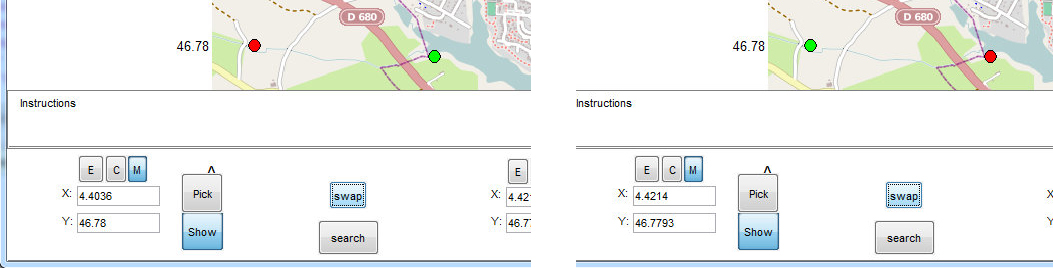
\includegraphics[ width=0.8\textwidth]{../pictures/724.jpg}
			  \caption{Yomap GUI "swap" button}
				\label{fig:724}
			  \end{figure}
									
			All possible information about points and way is represented in instruction panel (figure \ref{fig:725}).   
		  \begin{figure}[h]
		  \centering
		  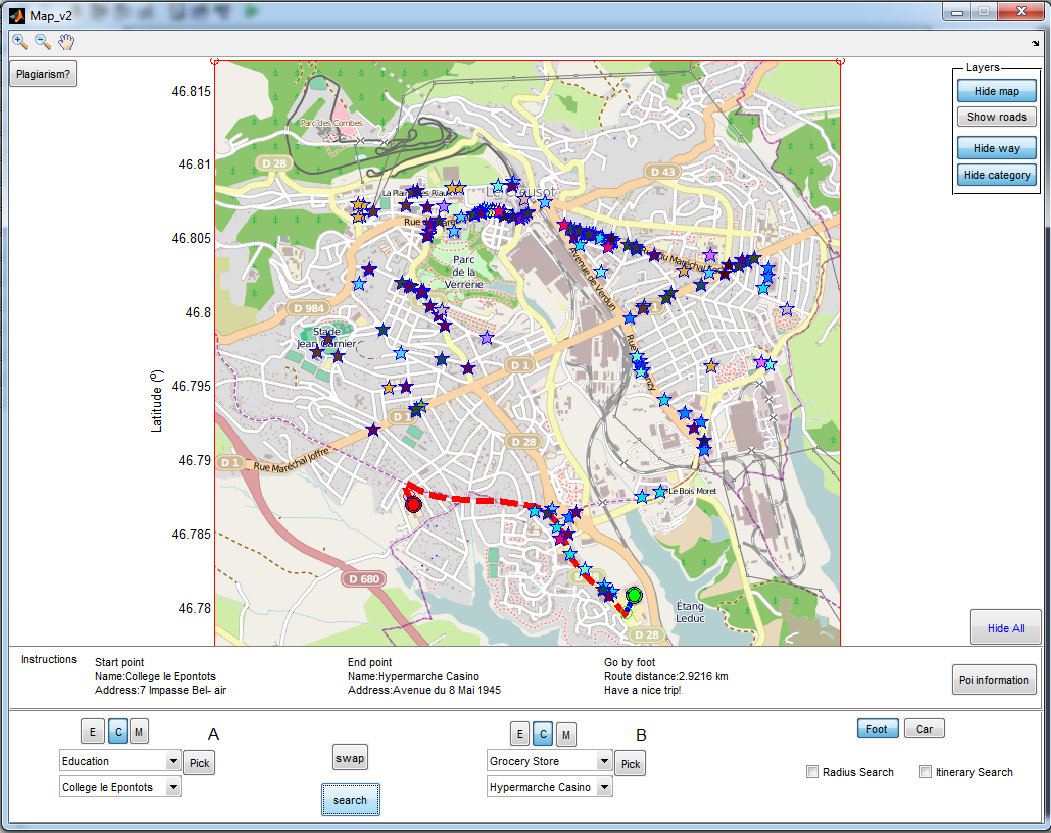
\includegraphics[ width=0.8\textwidth]{../pictures/725.jpg}
		  \caption{Yomap GUI instruction panel}
			\label{fig:725}
		  \end{figure}
			
			
		\subsubsection{Map Layers Plotting}
		Map by itself is complicated graphical structure that contains luck of information. That is why one of the biggest problems can appear in map representation is its overloading with information. So to prevent this and for user convenience we decide to use layers for plotting map. 
		Each layer represents only one type of information. In our GUI we have 4 main layers:
		\begin{itemize}
			\item Map Layer
			\item Roads Layer
			\item Way Layer
			\item Category Layer
		\end{itemize}
		
		Map layer (figure \ref{fig:726}) is a *.png image of map of Le Creusot that loads in the beginning of the program. 
		\begin{figure}[h]
		\centering
		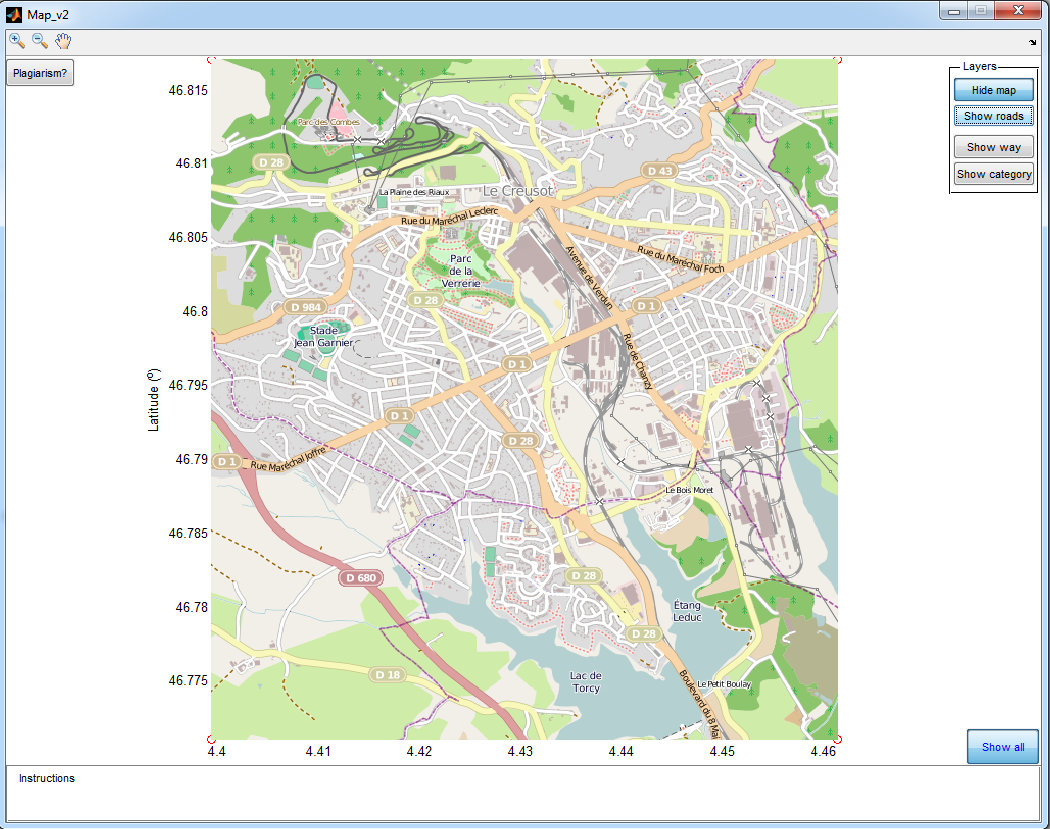
\includegraphics[ width=0.8\textwidth]{../pictures/726.jpg}
		\caption{Map layer}
		\label{fig:726}
		\end{figure}
		
		
		Roads layer (figure \ref{fig:727}) is a vector of location of nodes that we traverse in order to have way from point A to point B.
		\begin{figure}[h]
		\centering
		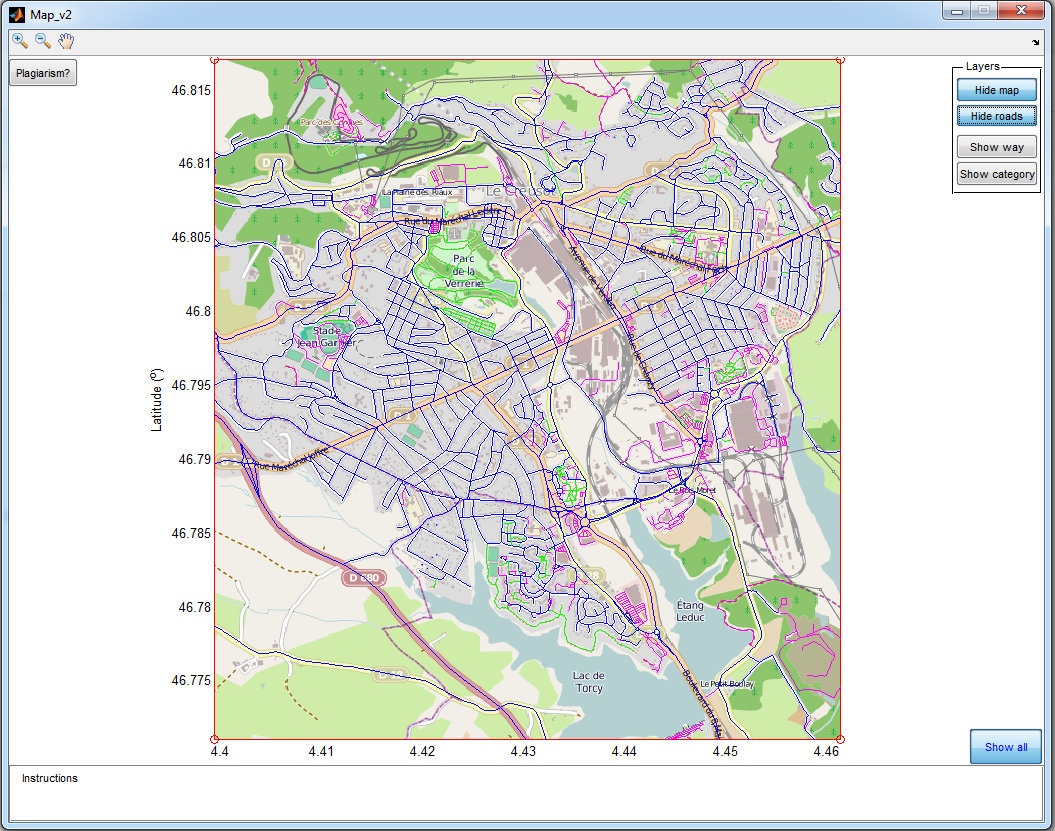
\includegraphics[ width=0.8\textwidth]{../pictures/727.jpg}
		\caption{Roads layer}
									\label{fig:727}
		\end{figure}
		
		Way layer (figure \ref{fig:728}) is a vector that shows the shortest way from point A to point B.
		\begin{figure}[h]
		\centering
		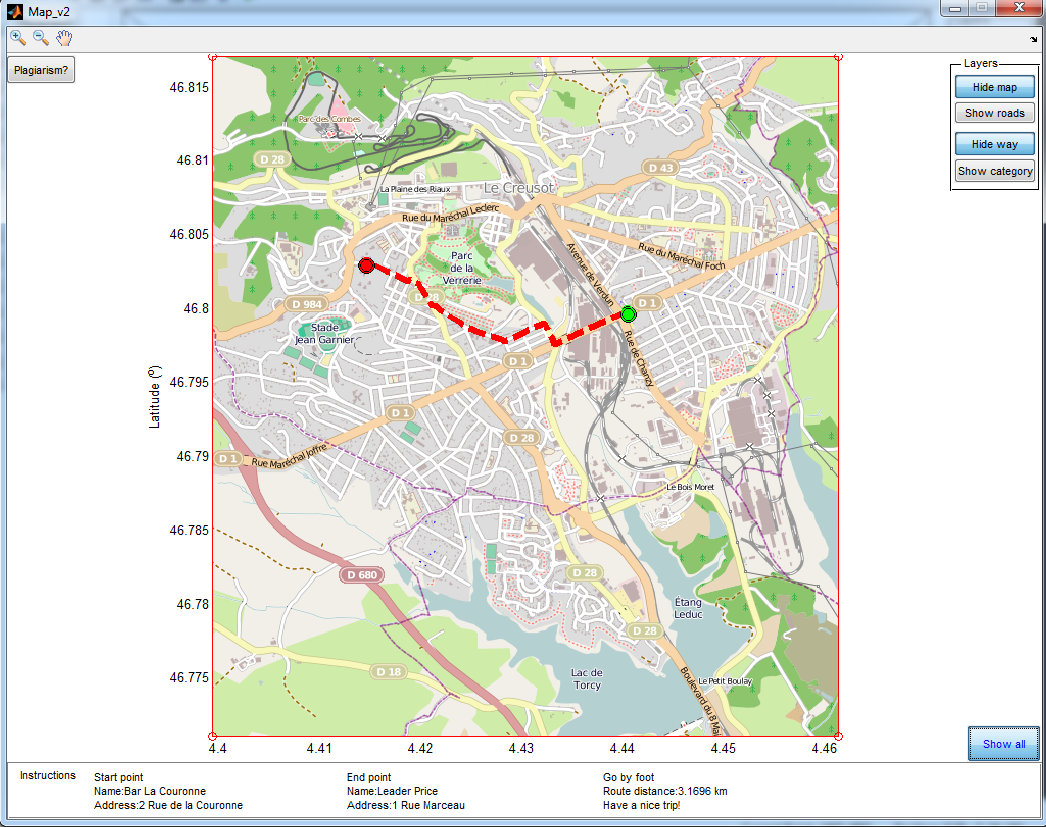
\includegraphics[ width=0.8\textwidth]{../pictures/728.jpg}
		\caption{Way layer}
		\label{fig:728}
		\end{figure}
		
		Category layer (figure \ref{fig:729}) is a representation of points of interest on the map.
		\begin{figure}[h]
		\centering
		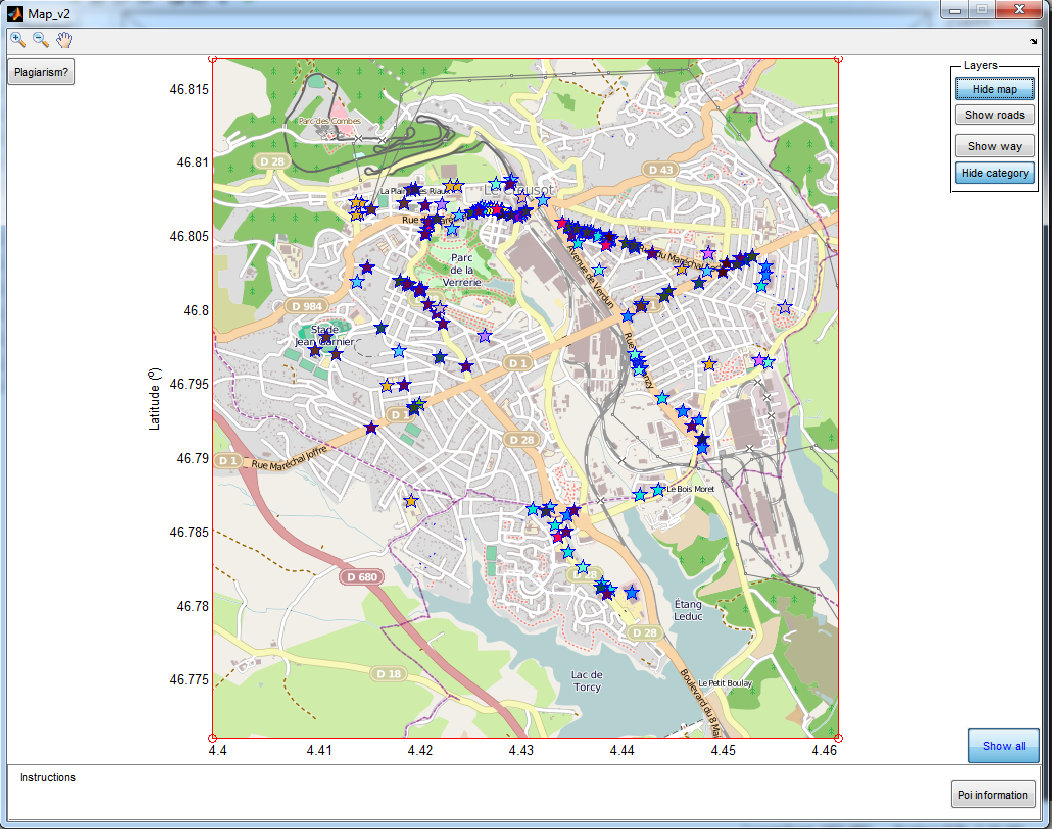
\includegraphics[ width=0.8\textwidth]{../pictures/729.jpg}
		\caption{Category layer}
		\label{fig:729}
		\end{figure}		
				
		Each layer can be shown either by itself either in a combination with others layers. Because MATLAB allows draw any graphics on each other in a row the function "map\_Show\_Result" was implemented. Any time if one of the layers buttons is pressed the function is called and conditions of all layers buttons are sent to it. Before any layer appeared function "prepareMap" is called. It allows preparing axes before drawing layers and after this depending on buttons value corresponding layer is drawn. Way layer can be drawn only in case if route between point A and B is found.
		
		\subsubsection{Mouse Click And Dots Plotting}
		As was already mentioned user is allowed to pick any point on the map using mouse. To pick any point MATLAB functions "WindowButtonDownFcn" and "get(handles.mapDraw,'currentpoint')" are used. Result of these functions returns coordinates of the axes at the place where mouse button was pressed (figure \ref{fig:7210}). 
		\begin{figure}[h]
		\centering
		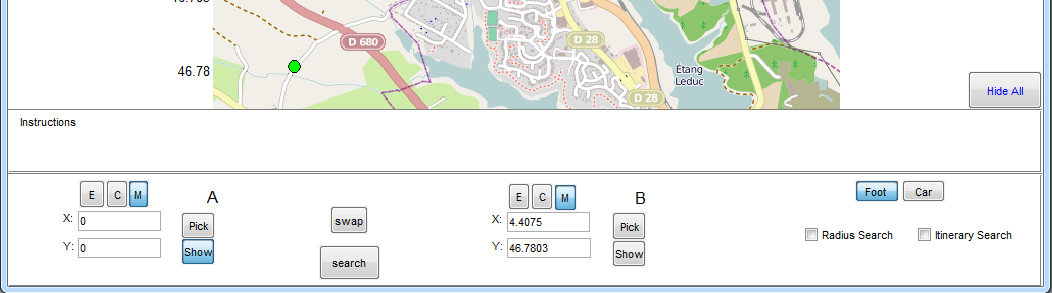
\includegraphics[ width=0.8\textwidth]{../pictures/7210.jpg}
		\caption{Mouse click}
		\label{fig:7210}
		\end{figure}		
		
		In case if user chooses "show on map" as a point representation then he allows to take any point on the map even if "show category" button pressed. In case if "show category" button pressed but user choose "category search" or "search by enter" then he can pick only category points, otherwise point could not be plotting and data could not be saved. Any points that picked on the map are checked on being not out of range (figure \ref{fig:7211}).
 
		\begin{figure}[h]
		\centering
		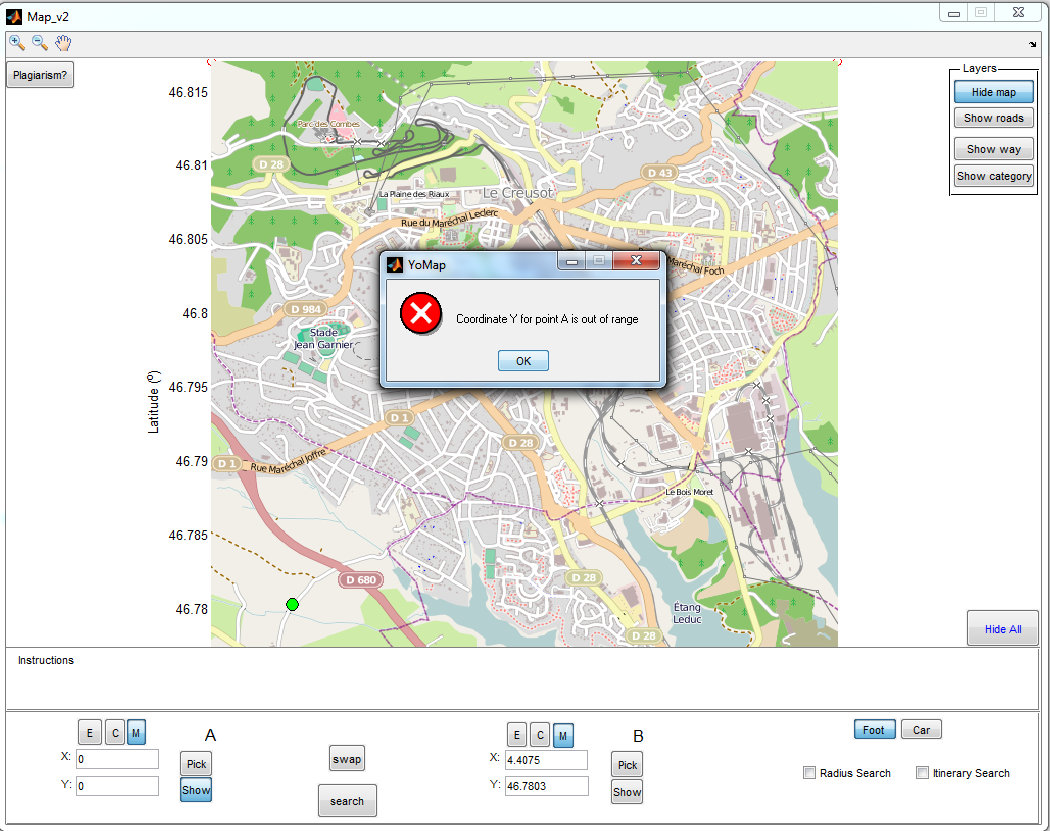
\includegraphics[ width=0.8\textwidth]{../pictures/7211.jpg}
		\caption{Out of range checking}
		\label{fig:7211}
		\end{figure}			
		
		Dots plotting after mouse click is the most difficult and "unstable" layer. The problem is in plotting dots for every point with saving map layers. We should always take into account how many points do we have, which of them are already plotted, which we need to plot and etc. 
		To solve this problem we used flag and handle to each point. Flag allows us to check if point already plotted or not and handle is used for deleting/plotting dot. For plotting dots function "draw\_point" was implemented. 
		To avoid problems with plotting points and layers algorithm that shown on figure 7212 was developed. It allows to draw any point on any layer independently.
 
		\begin{figure}[h]
		\centering
		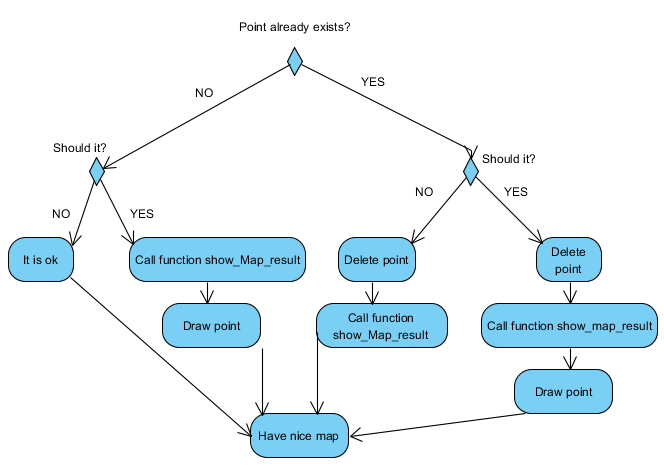
\includegraphics[ width=0.8\textwidth]{../pictures/7212.jpg}
		\caption{Dots plotting algorithm}
		\label{fig:7212}
		\end{figure}
